\documentclass{article}
\usepackage[utf8]{inputenc}
\usepackage{graphicx}

\title{Python}


\begin{document}

\maketitle

\section{Sejarah Python}
Python yang didirikan Guido van Rossum pertama di Centrum Wiskunde dan Informatica (CWI) Belanda pada tahun 1990. Python yang terinspirasi dari Bahasa ABC. Hingga sekarang, Guido menjadi penulis utama pada python.
Di tahun 1995, Guido meneruskan pembuatan Python di Corporation for National Research Initiative(CNRI) di Virginia Amerika. Pada Mei 2000, Guido and Team Python pinda menuju BeOpen.com dan dilanjutkan membentuk tim BeOpen PythonLabs.
Python dibagi beberapa versi yaitu\\
•	Python 1.0-Januari 1994\\
o	Python 1.2 – 10 April 1995\\
o	Python 1.3 – 12 Oktober 1995\\
o	Python 1.4 – 25 Oktober 1996\\
o	Python 1.5 – 31 Desember 1997\\
o	Python 1.6 – 5 September 2000\\
•	Python 2.0-Oktober 2000\\
o	Python 2.1 – 17 April 2001\\
o	Python 2.2 – 21 Desember 2001\\
o	Python 2.3 – 29 Juli 2003\\
o	Python 2.4 – 30 Nopember 2004\\
o	Python 2.5 – 19 September 2006\\
o	Python 2.6 – 1 Oktober 2008\\
o	Python 2.7 – 3 Juli 2010\\
•	Python 3.0-Desember 2008\\
o	Python 3.1 – 27 Juni 2009\\
o	Python 3.2 – 20 Februari 2011\\
o	Python 3.3 – 29 September 2012\\
o	Python 3.4 – 16 Maret 2014\\
o	Python 3.5 – 13 September 2015\\
o	Python 3.6 – 23 Desember 2016\\
o	Python 3.7 – 27 Juni 2018\\
\section{Sejarah Pyhton}
	Python kembangkan oleh Guido van Rossum pada tahun 1990 di CWI. Amsterdam kelanjutan dari bahasa pemrograman ABC.Versi yang terakhir dari CWI 1.2 tahun 1995, Guido pindah ke CNRI versi yang dikeluarkan 1.6 tahun 2000. Guido dan pengembang inti pindah ke BeOpen.com perusahaan komersial dan membentuk BeOpen PythonLabs dengan versi 2.0. Guido Pindah ke DigitalCreations. sekumpulan pemrograman yang dikoordinir Guido dan Python Software Foundation. Software Foundation adalah sebuah organisasinon-profit dengan versi 2.1 dan mencegah Python dimiliki oleh perusahaan komersial. Saat ini Pyhton sudah mencapai versi 2.7.13 dan versi 3.6.0.
\section{Perbedaan Python 2 dan 3}
	Perbedaan yang pertama adalah :\\
	\textbf{1. Syntax untuk mencetak teks}\\
	Di Pyhton 2 perintah print menggunakan tandakurung dan tidak menggunakan  kurung juga bisa di jalankan, contoh:\\
	\\
	print"Tidak Memakai kurung"\\
	print("Memakai Kurung")\\
	print"ini,;print"satu baris"\\
	\\
	Di Python 3 perintah print harus menggunakan tanda kurung, contoh:\\
	\\
	print("Menggunakan Kurung")\\
	print("digunakan untuk",end=")\\
	print("satu baris")\\
	\\
	\textbf{2. Syntax Input}\\
	Di Python 2 pada pemberian syntax input menggunakan raw dan menggunakan kutip satu,setelah itu print tidak memakai kurung contoh:\\
	\\
	 nama=raw\textunderscore input('Nama Anda:')\\
	 print nama\\
	 \\
	 di Python 3 pada pemberian syntax iput menggunakan kutip dua dan tidak menggunakan raw. setelah itu print menggunakan tanda kurung, contoh:\\
	 \\
	 nama=input("Nama Anda:")\\
	 print(nama)\\
	 \textbf{3. Hasil Pembagian}\\
	 Di Python 2 setelah print tidak menggunakan tanda kurung. contoh:\\
	 \\
	 print "3 / 2 = " , 3/2\\
	 print "3 // 2 = " , 3//2\\
	 \\
	 Di Python 3 setelah print menggunakan tanda kurung. contoh :\\
	 \\
	 print ("3 / 2 = " , 3/2)\\
	 print ("3 // 2 = " , 3//2)\\
\subsection{Python di Perusahaan Dunia}
\subsubsection{Google}
Dari awal berdiri, Google sudah menggunakan Python, bahkan Python merupakan salah satu bahasa pemrograman yang penting bagi Google, itulah mengapa Google pernah merekrut kreator Python Guido Van Rossum untuk bekerja di Google.\\

\noindent Sebuah kutipan dari pendiri Google “Python where we can, C++ where we must,” kutipan ini artinya jika menginginkan kontrol akan memori dan latensi yang rendah maka gunakan C++, sisanya gunakan Python sebisa mungkin, meskipun ada script yang ditulis untuk Google dalam bahasa Perl atau Bash, nantinya script tersebut akan diubah lagi ke Python, alasannya adalah karena kemudahan dalam perawatan.\\

\noindent Saat ini Python merupakan salah satu bahasa pemrograman server-side resmi di Google, selain Pyhton Google juga menggunakan C++, Java dan Go.
\\
\\
\\
\\
\\
\\
\\
\\
\\
\\
\\
\\
\\
\\

\section{Instalasi}
\subsection{Anaconda 3}
1. Buka Setup Anaconda 3 and pencet next\\
\begin{figure}[h]
	\centering
		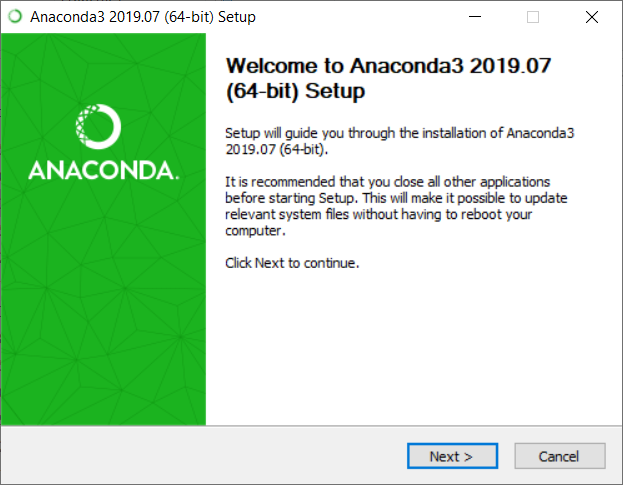
\includegraphics[scale=0.5]{Gambar/A1.PNG}
		\caption{setup Anaconda 3}
\end{figure}

2. Klik I Agree\\
\begin{figure}[h]
	\centering
		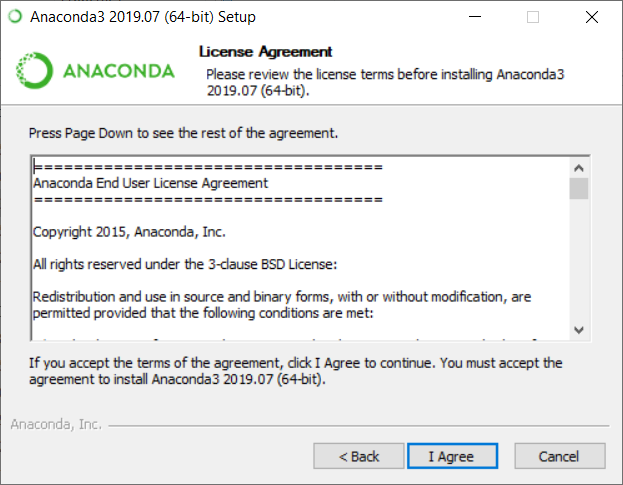
\includegraphics[scale=0.5]{Gambar/A2.PNG}
		\caption{setup Anaconda 3}
\end{figure}

3. Klik Just Me, and lanjut Klik Next\\
\begin{figure}[h]
	\centering
		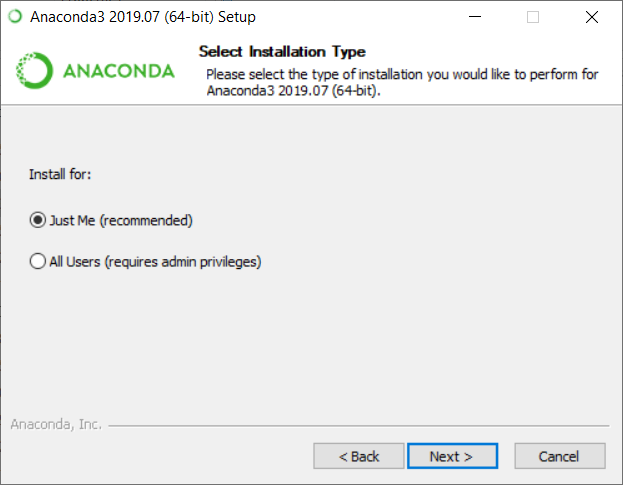
\includegraphics[scale=0.5]{Gambar/A3.PNG}
		\caption{Setup Anaconda 3}
\end{figure}
\\
\\
\\
\\
\\
\\
\\
\\
4. Simpan Data Anaconda di folder C\\
\begin{figure}[h]
	\centering
		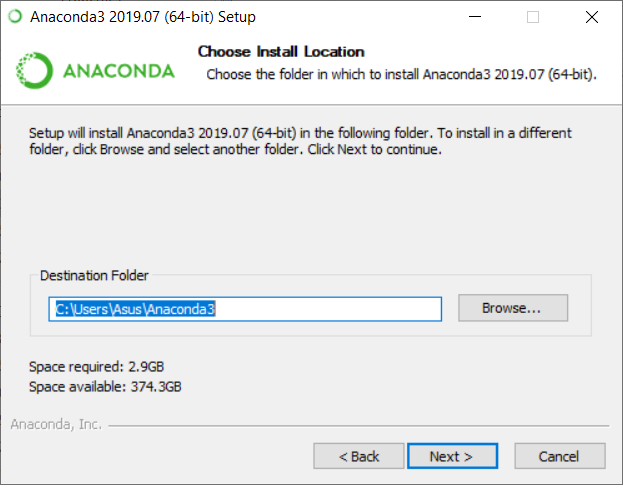
\includegraphics[scale=0.5]{Gambar/A4.PNG}
		\caption{Setup Anaconda 3}
\end{figure}
\\
\\
\\
\\
\\
\\
\\
\\
5. Pilihlah kedua Pilihan yang ada di instalasi Anaconda\\
\begin{figure}[h]
	\centering
		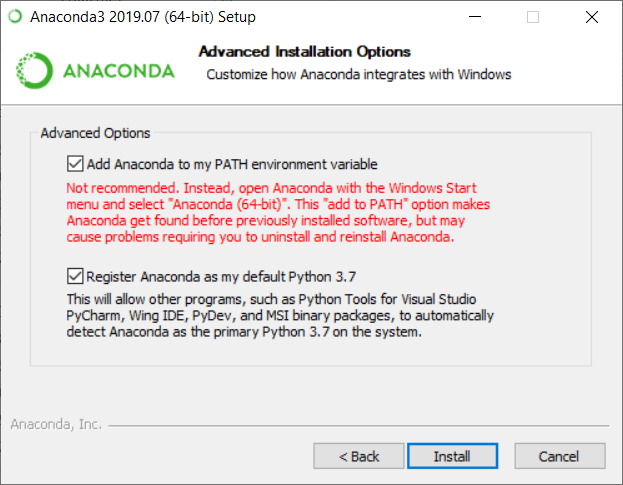
\includegraphics[scale=0.5]{Gambar/A5.PNG}
		\caption{Setup Anaconda 3}
\end{figure}
\\
\\
\\
\\
\\
\\
\\
\\
6. Tunggu hingga proses instalasi selesai\\
\begin{figure}[h]
	\centering
		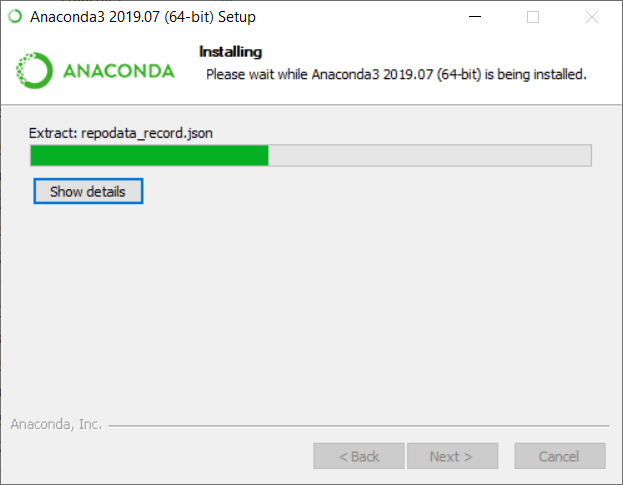
\includegraphics[scale=0.5]{Gambar/A6.PNG}
		\caption{Setup Anaconda 3}
\end{figure}
\\
\\
\\
\\
\\
\\
\\
\\
7. Klik Next seperti gambar\\
\begin{figure}[h]
	\centering
		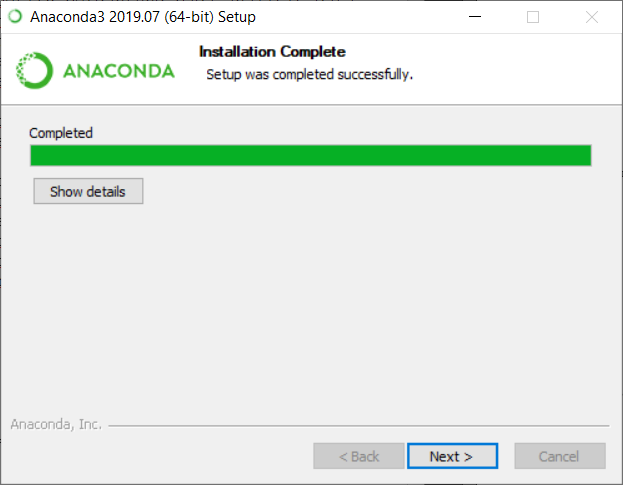
\includegraphics[scale=0.5]{Gambar/A7.PNG}
		\caption{Setup Anaconda 3}
\end{figure}
\\
\\
\\
\\
\\
\\
\\
\\
8.Klik next seperti gambar\\
\begin{figure}[h]
	\centering
		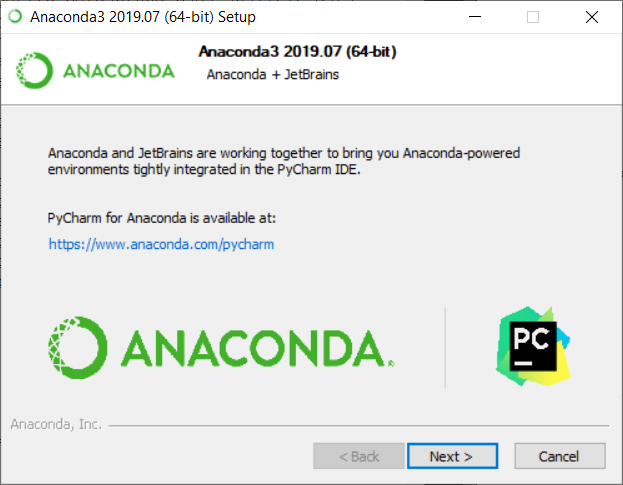
\includegraphics[scale=0.5]{Gambar/A8.PNG}
		\caption{Setup Anaconda 3}
\end{figure}
\\
\\
\\
\\
\\
\\
\\
\\
\\
\\
\\
\\
\\
9. Klik Finish ketika instalasi selesai\\
\begin{figure}[h]
	\centering
		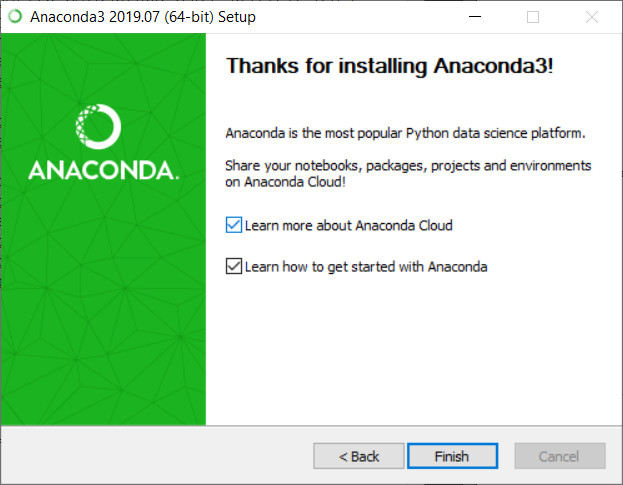
\includegraphics[scale=0.5]{Gambar/A9.PNG}
		\caption{Setup Anaconda 3}
\end{figure}
\subsection{ pip.py }
1. Buka CMD dan ketik cd desktop
\begin{figure}[h]
	\centering
		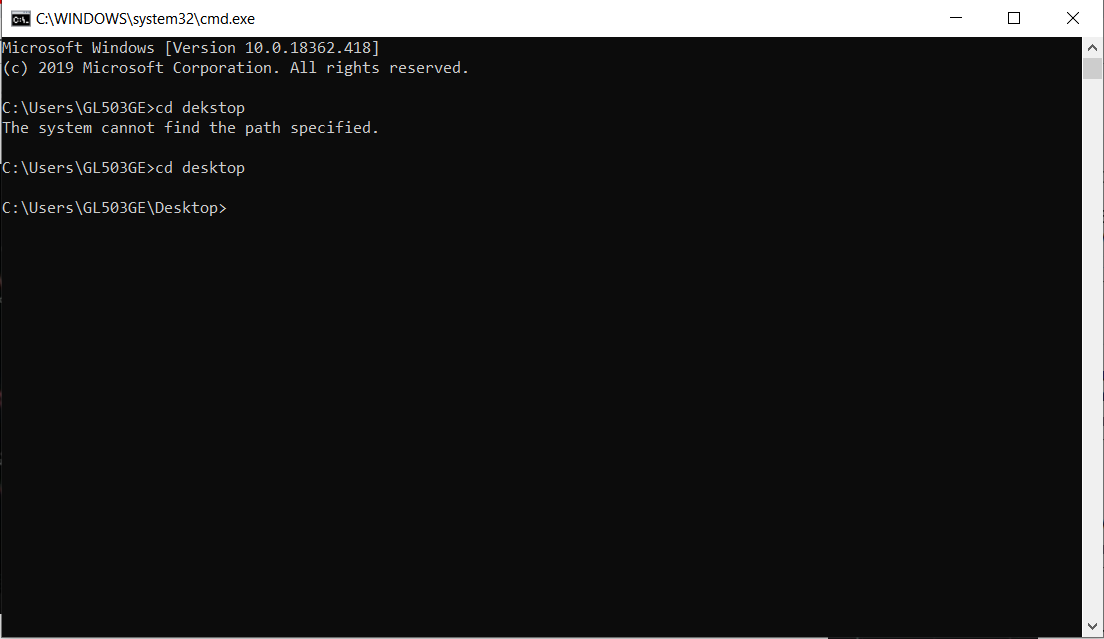
\includegraphics[scale=0.5]{Gambar/B1.PNG}
		\caption{Setup Anaconda 3}
\end{figure}
\\
\\
\\
\\
\\
\\
\\
\\
\\
\\
\\
\\
\\
\\
\\
2. setelah masuk ke direktori Desktop, Ketik Python get-pip.py
\begin{figure}[h]
	\centering
		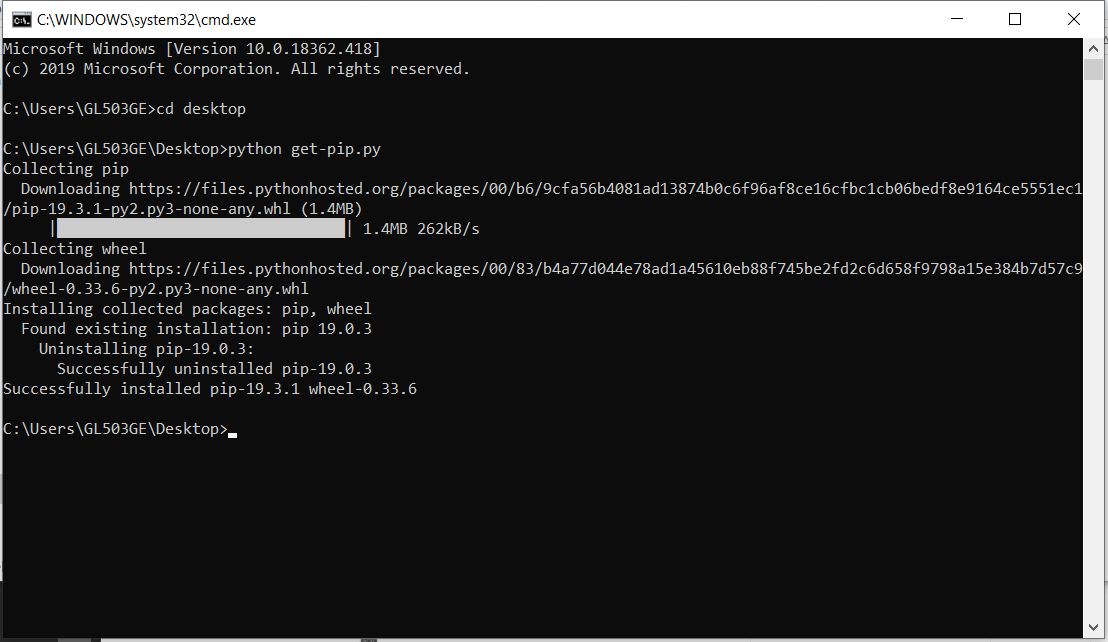
\includegraphics[scale=0.5]{Gambar/B2.PNG}
		\caption{Setup Anaconda 3}
\end{figure}
\\
\\
\\
\\
\\
\\
\\
\\
\\
\\
\\
\\
\\
\\
\\
\\
\\
\\
\\
\\
\\
\subsection{cara setting environment }
\subsection{mencoba entrepreter/cli melakui terminal atau cmd windows}
1. Buka Cmd dan ketik Python
\begin{figure}[h]
	\centering
		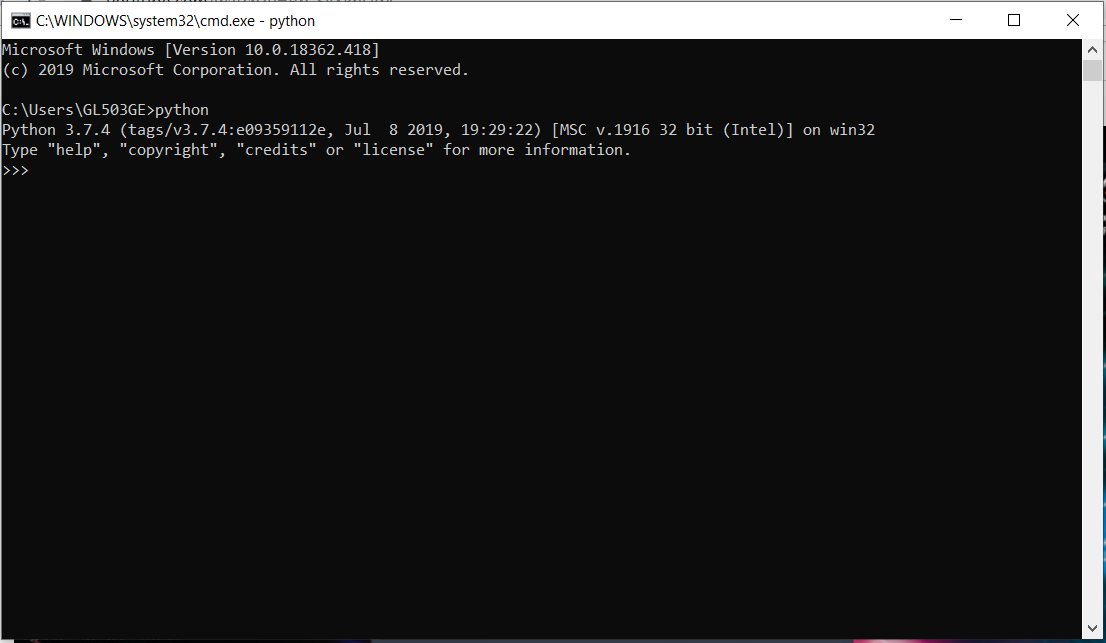
\includegraphics[scale=0.5]{Gambar/C1.PNG}
		\caption{Setup Anaconda 3}
\end{figure}
\\
\\
\\
\\
\\
\\
\\
\\
\\
\\
\\
\\
\\
\\
\\
\\
\\
\\
\\
\\
\\
\\
\\
\\
\\
\\
2. Untuk mencoba perintah Input, ketik "input("Nama Anda: ")
\begin{figure}[h]
	\centering
		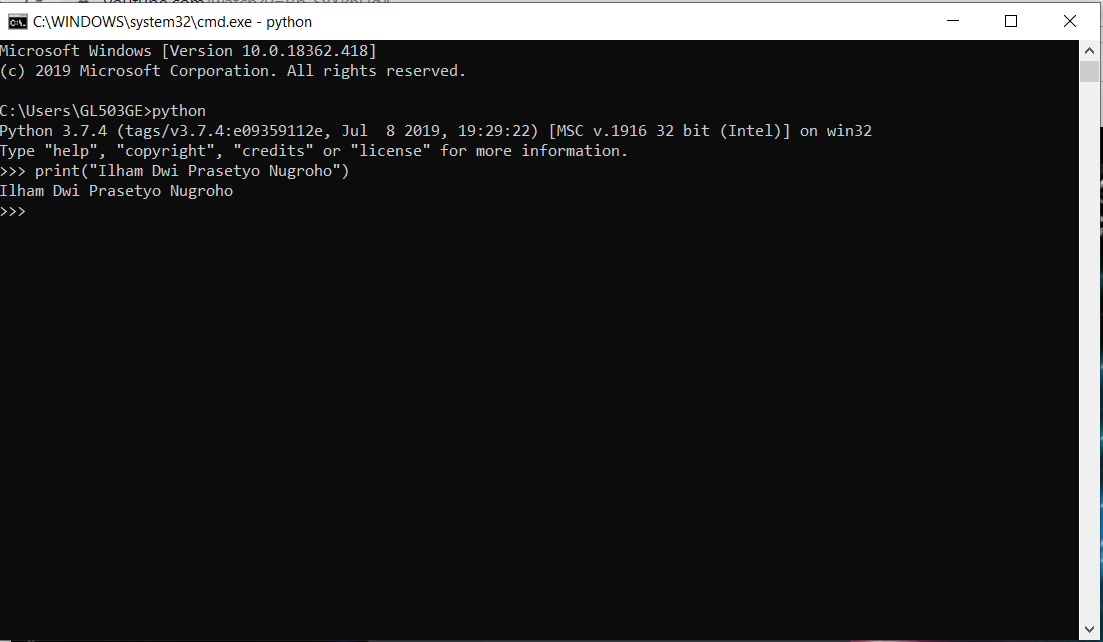
\includegraphics[scale=0.5]{Gambar/C2.PNG}
		\caption{Setup Anaconda 3}
\end{figure}
\\
\\
\\
\\
\\
\\
\\
\\
\\
\\
\\
\\
\\
\\
\\
\\
\\
\\
\\
\\
\\
\\
\\

3. Untuk memberi perintah matematika perkalian, ketik "4*4" dan tekan enter
\begin{figure}[h]
	\centering
		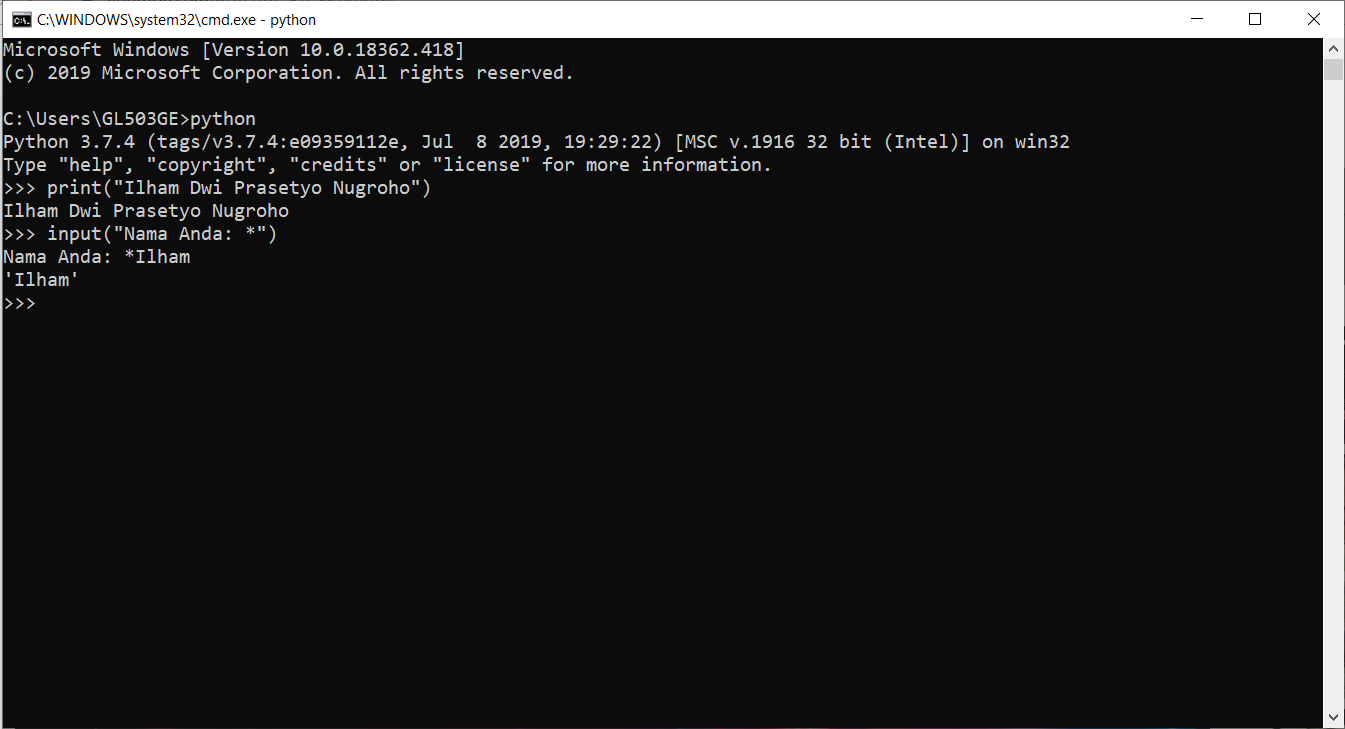
\includegraphics[scale=0.5]{Gambar/C3.PNG}
		\caption{Setup Anaconda 3}
\end{figure}
\\
\\
\\
\\
\\
\\
\\
\\
\\
\\
\\
\\
\\
\\
\\
\\
\\
\\
\\
\\
\\
\\
\\
\\
\\
\\
\subsection{Menjalankan dan mengupdate anaconda dan spyder}
1. Buka cmd dan ketik "conda install -c anaconda python
\begin{figure}[h]
	\centering
		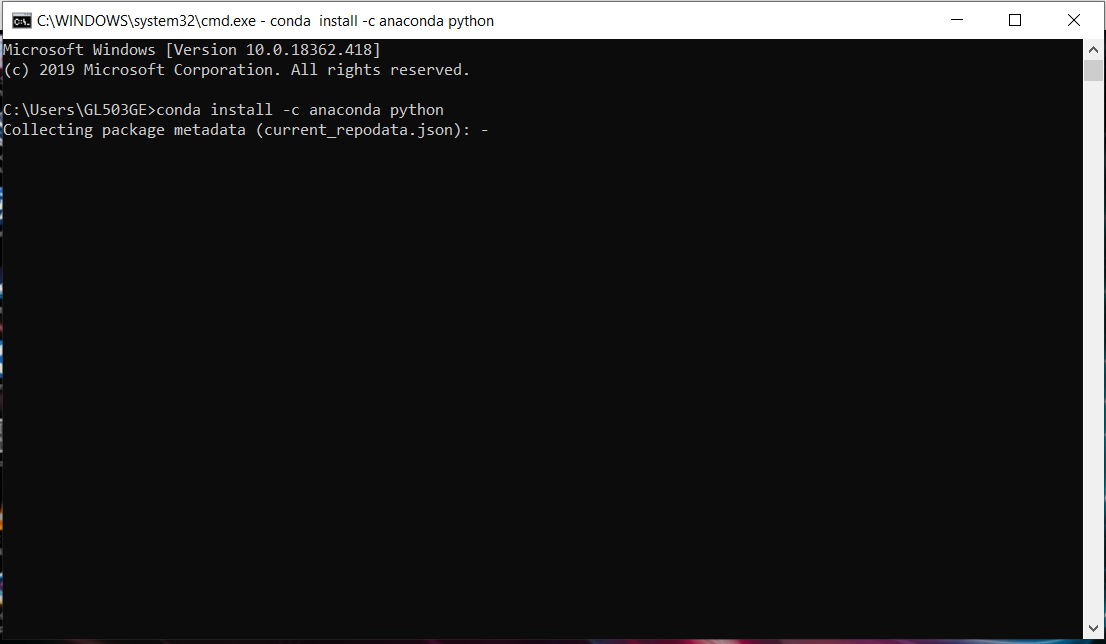
\includegraphics[scale=0.5]{Gambar/D1.PNG}
		\caption{Setup Anaconda 3}
\end{figure}
\\
\\
\\
\\
\\
\\
\\
\\
\\
\\
\\
\\
\\
\\
\\
\\
\\
\\
\\
\\
\\
\\
\\
\\
\\
\\
2. Ketik huruf y untuk melanjutkan
\begin{figure}[h]
	\centering
		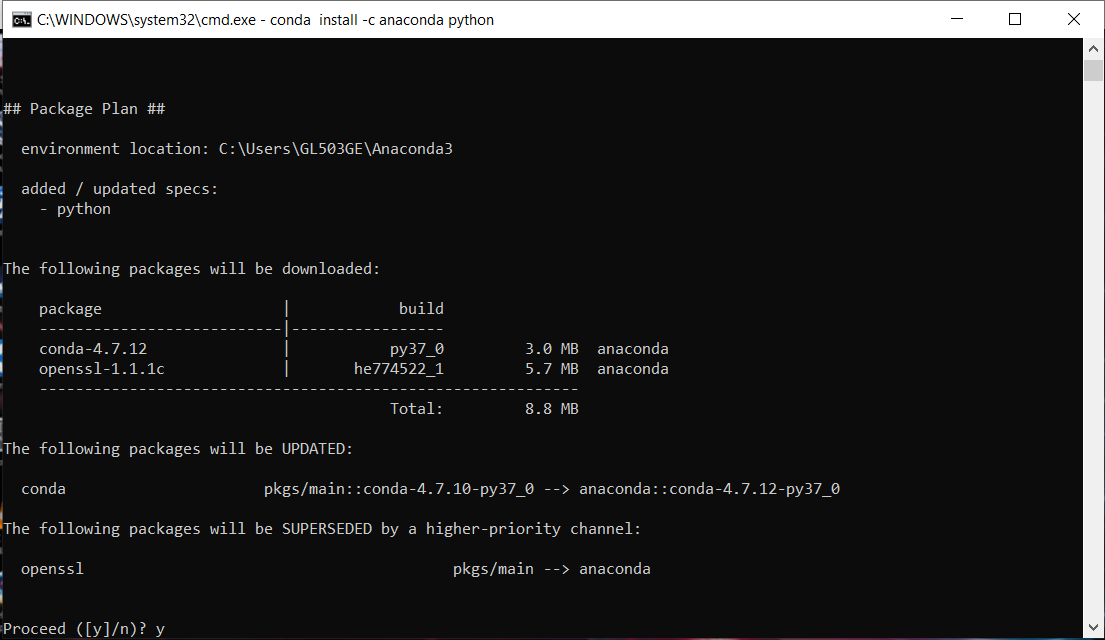
\includegraphics[scale=0.5]{Gambar/D2.PNG}
		\caption{Setup Anaconda 3}
\end{figure}
\\
\\
\\
\\
\\
\\
\\
\\
\\
\\
\\
\\
\\
\\
\\
\\
\\
\\
\\
\\
\\
\\
\\
\\
\\
\\
3. setelah selesai, akan tampil seperti ini
\begin{figure}[h]
	\centering
		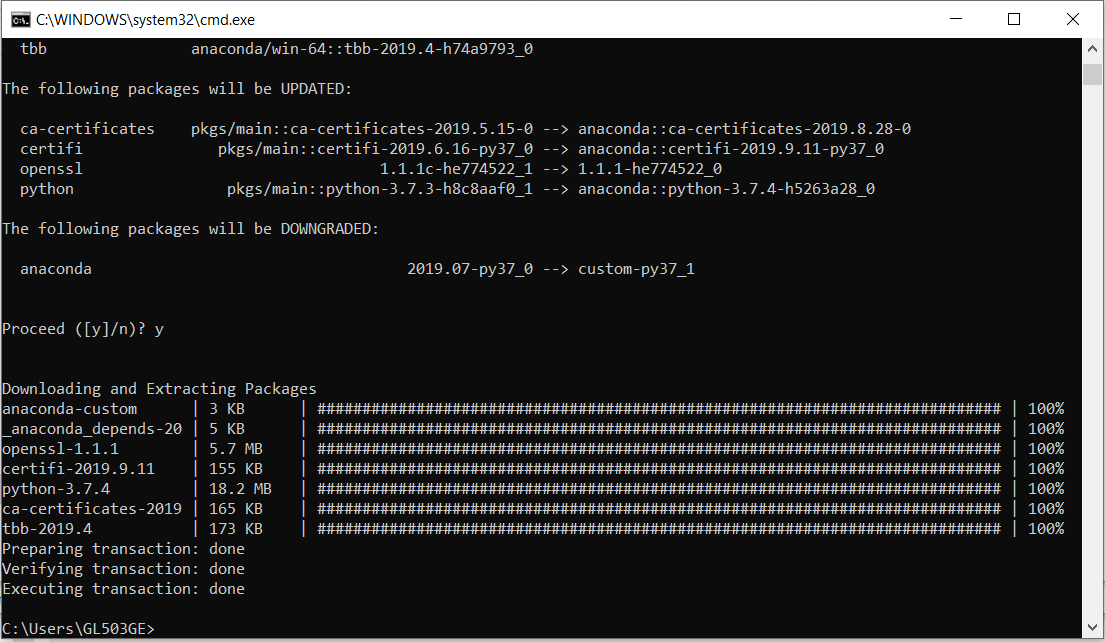
\includegraphics[scale=0.5]{Gambar/D3.PNG}
		\caption{Setup Anaconda 3}
\end{figure}
\\
\\
\\
\\
\\
\\
\\
\\
\\
\\
\\
\\
\\
\\
\\
\\
\\
\\
\\
\\
\\
\\
\\
\\
\\
\\

\section{Menjalankan Script Hello World di Spyder}
1. Buka Anaconda 3 , Lalu pilih Launch Sypder.\\
\begin{figure}[h]
	\centering
		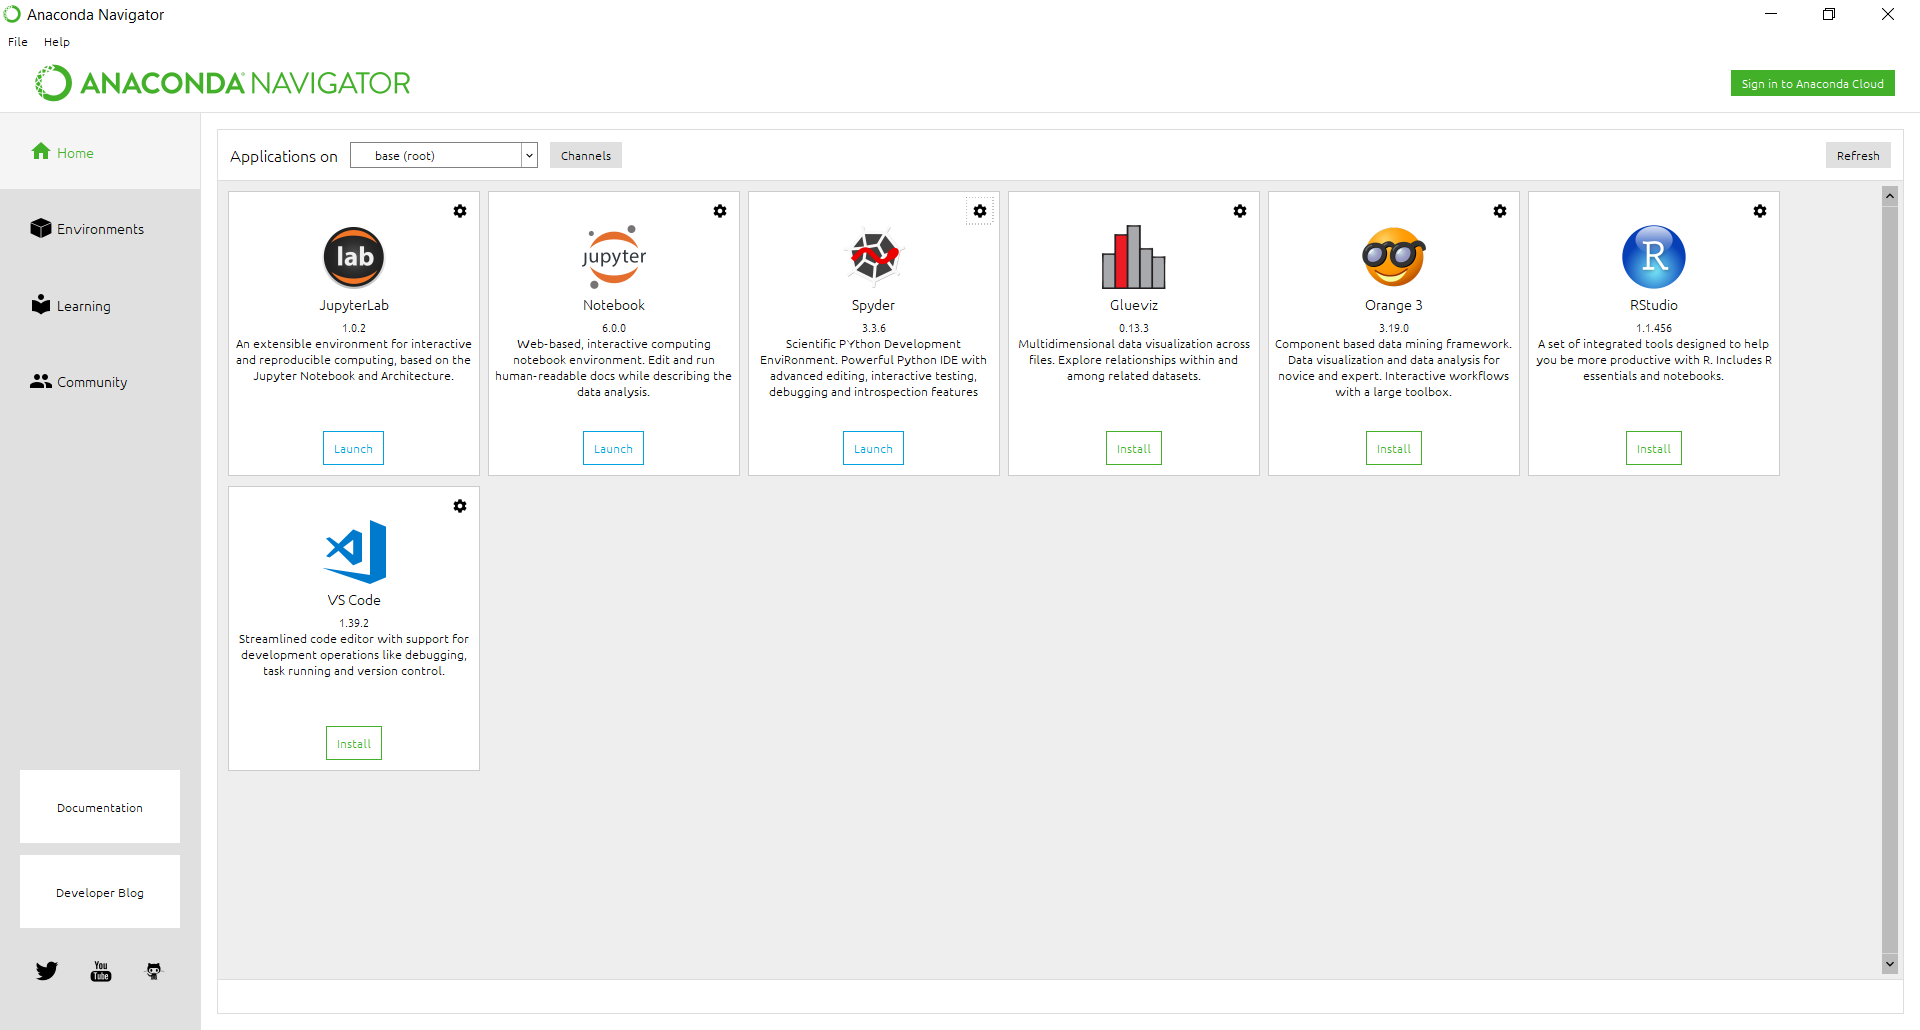
\includegraphics[scale=0.2]{Gambar/S1}
		\caption{Spyder}
\end{figure}
\\
\\
\\
\\
\\
\\
\\
\\
\\
\\
\\
\\
\\
\\
\\
\\
\\
\\
\\
\\
\\
\\
\\
\\
\\
\\
\\
2. Ketik seperti dibawah ini, lalu Klik Run.\\
\begin{figure}[h]
	\centering
		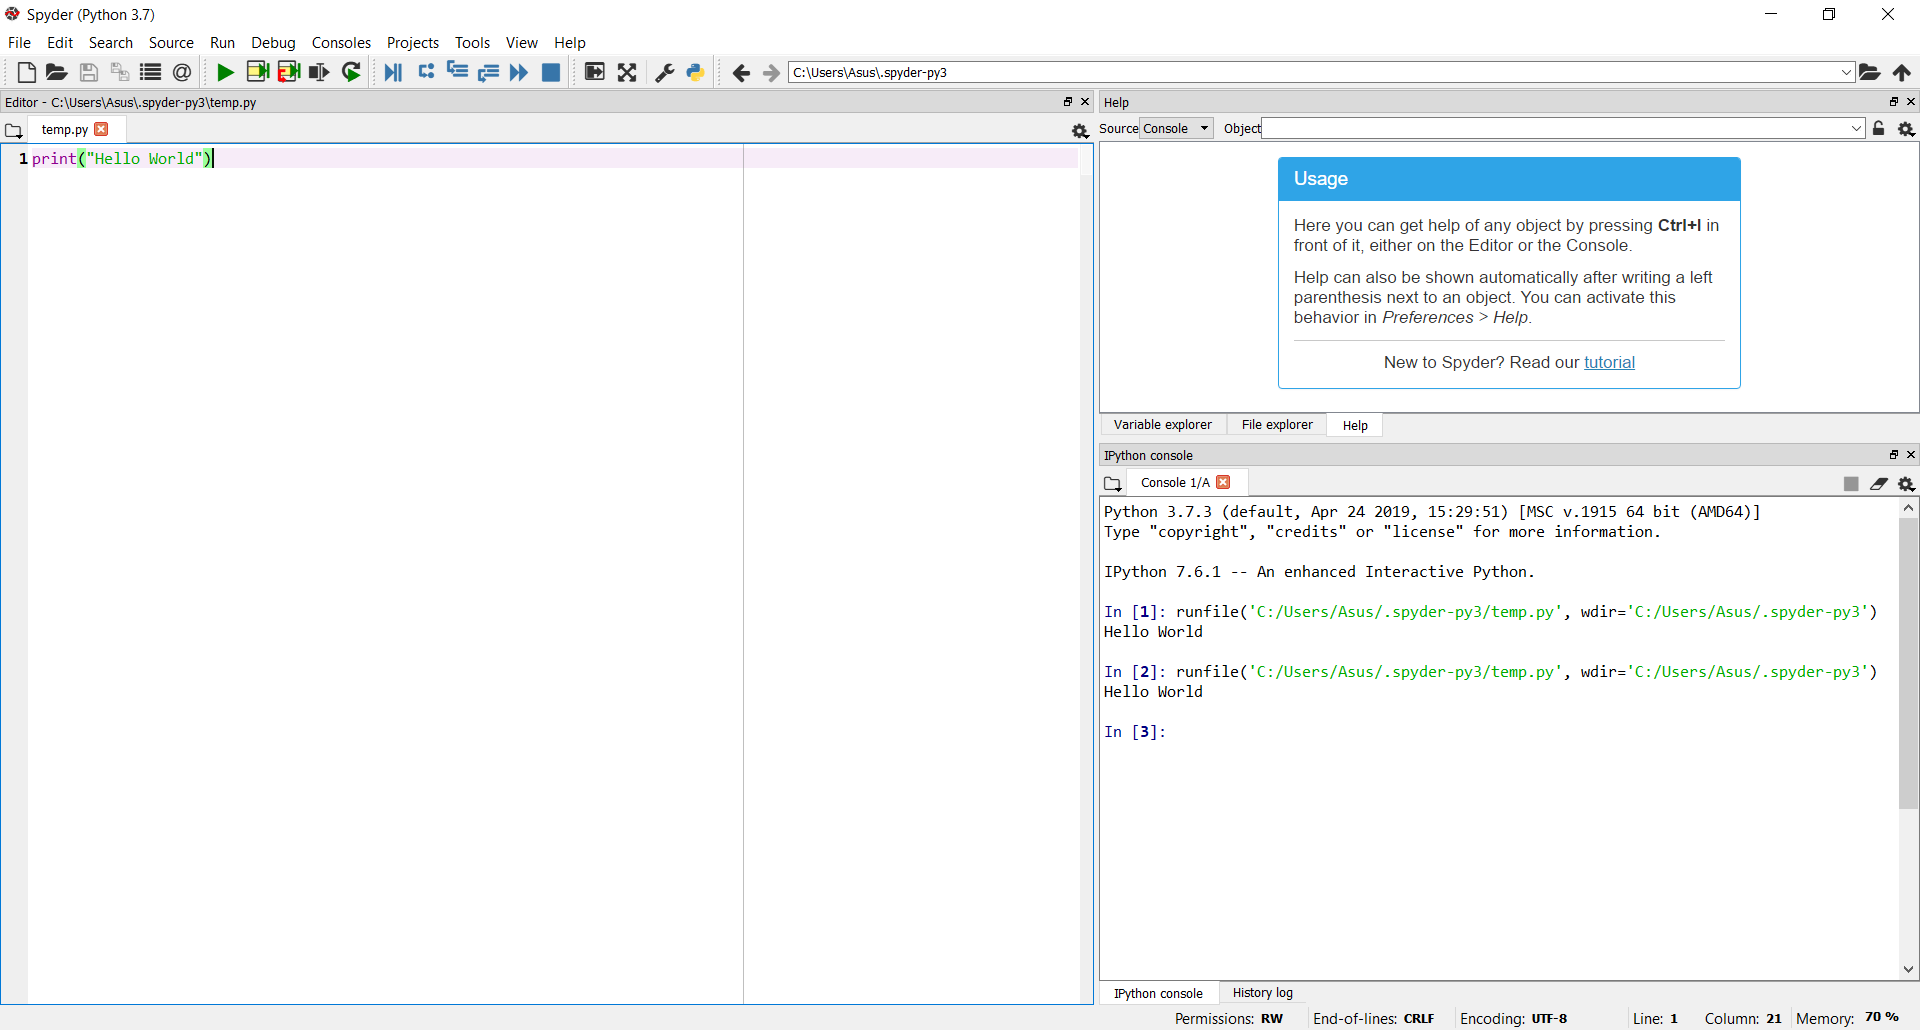
\includegraphics[scale=0.2]{Gambar/S2}
	\caption{Hellow World}
\end{figure}
\\
\\
\\
\\
\\
\\
\\
\\
\\
\\
\\
\\
\\
\\
\\
\\
\\
\\
\\
\\
\\
\\
\\
\\
\\
\\
\section{Cara menjalankan Script otomatis login aplikasi akademik dengan library selenium dan inputan user}

\section{Cara pemakaian variable explorer di spyder}
1. Buka Spyder\\
2. Ketikan Seperti di gambar ini\\
\begin{figure}[h]
	\centering
		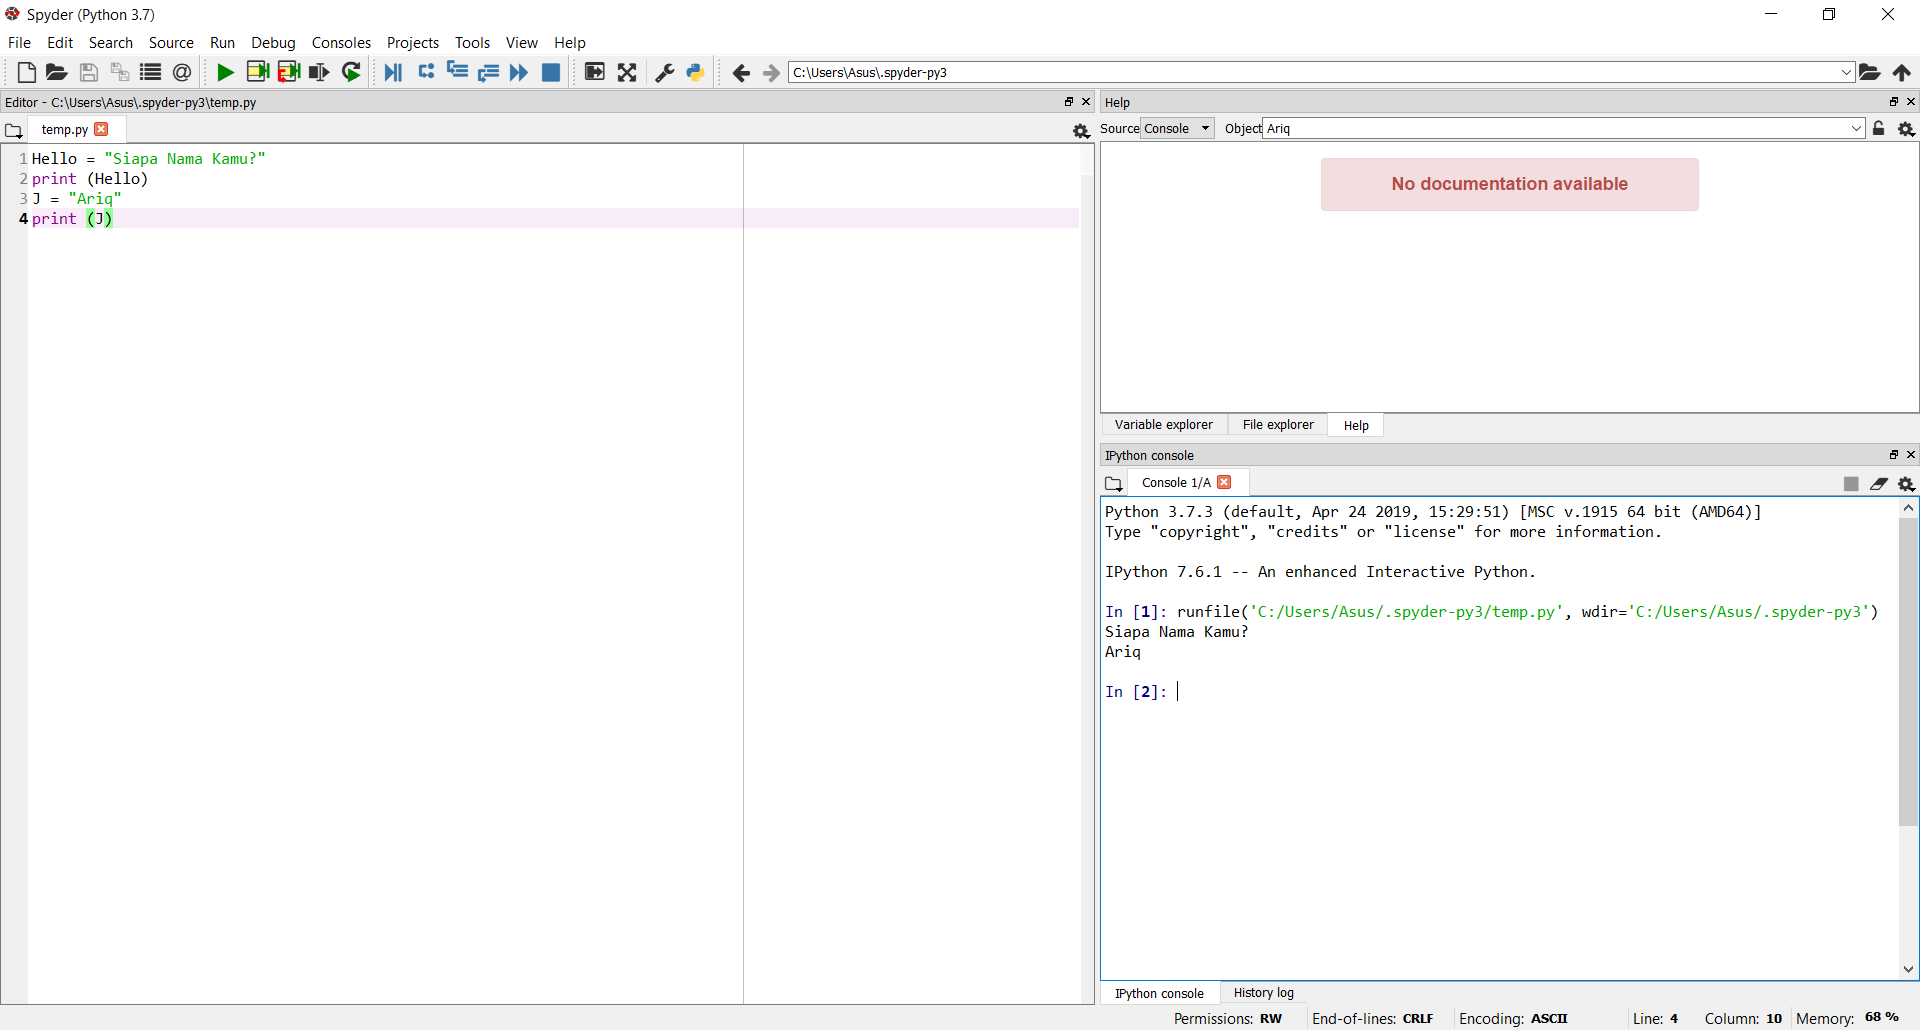
\includegraphics[scale=0.2]{Gambar/V1}
	\caption{Variable}
\end{figure}
\\
\\
\\
\\
\\
\\
\\
\\
\\
\\
\\
\\
\\
\\
\\
\\
\\
\\
\\
\\
\\
\\
\\
\\
\\
\\
\\
\section{Penjelasan Identasi}
Identasi adalah bagian dari suatu paragraf yang menjorok kedalam pada baris tiap paragraf. Mengatur indentasi dengan cara menggunakan tab atau spasi. Identasi digunakan oleh bahasa pemrograman python sebagai pengganti briket () untuk membuka dan menutup suatu fungsi. Error indentasi dapat terjadi jika syntax tidak menggunakan tab atau space.

\section{jenis jenis error identasi yang didapat}
1. Jenis codingan yang menjorok kedalam , dapat menyebabkan error.\\
\begin{figure}[h]
	\centering
		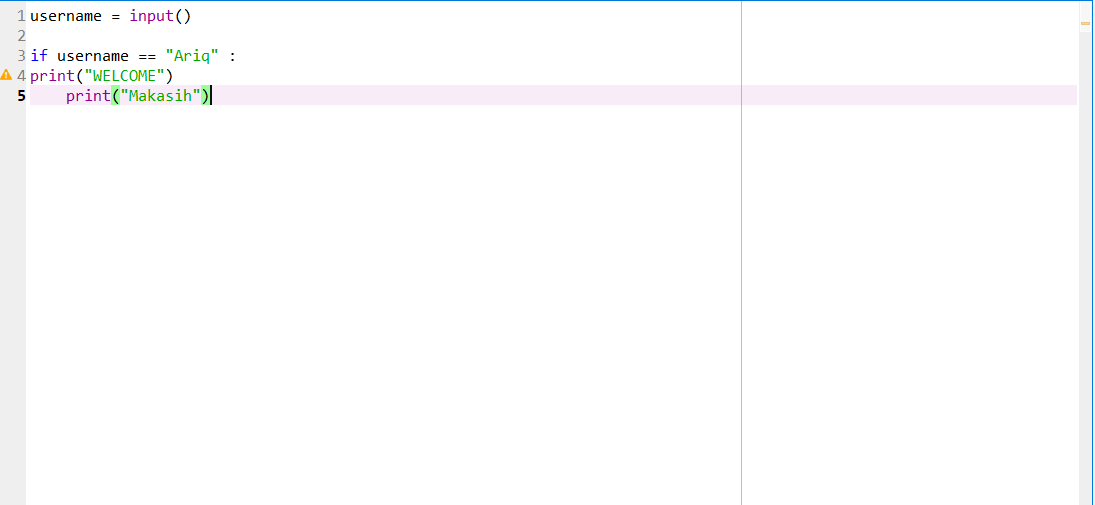
\includegraphics[scale=0.4]{Gambar/E1}
	\caption{Error1}
\end{figure}
\\
\\
\\
\\
\\
\\
\\
\\
\\
\\
\\
\\
\\
\\
\\
\\
\\
\\
\\
\\
\\
\\
\\
\\
\\
\\
\\
2. Run Program , maka hasilnya 	Error\\
\begin{figure}[h]
	\centering
		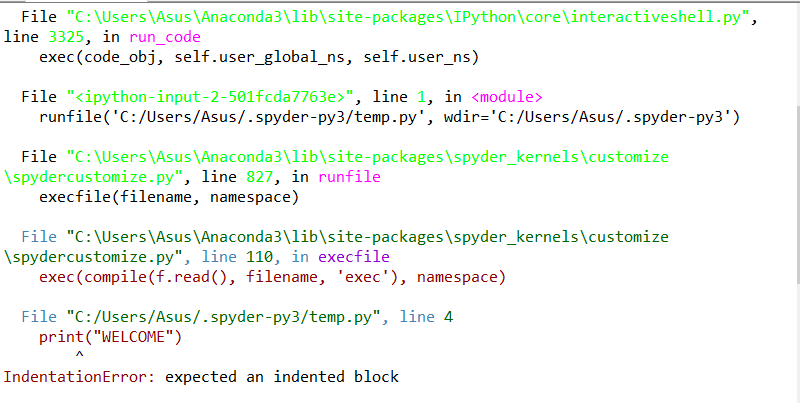
\includegraphics[scale=0.5]{Gambar/E2}
	\caption{Error2}
\end{figure}
\\
\\
\\
\\
\\
\\
\\
\\
\\
\\
\\
\\
\\
\\
\\
\\
\\
\\
\\
\\
\\
\\
\\
\\
\\
\\
\\
\section{cara membaca error}
1. Coding yang tidak bisa di run, dan ada tanda warning di samping.
\begin{figure}[h]
	\centering
		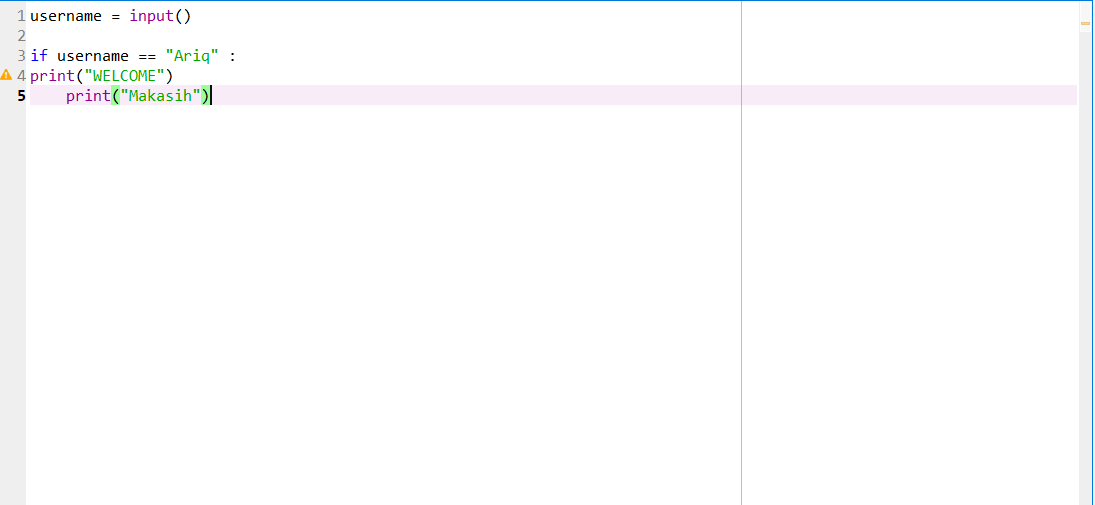
\includegraphics[scale=0.4]{Gambar/E1}
	\caption{Membaca error}
\end{figure}
\\
\\
\\
\\
\\
\\
\\
\\
\\
\\
\\
\\
\\
\\
\\
\\
\\
\\
\\
\\
\\
\\
\\
\\
\\
\\
\\
2. Maka akan tulisan seperti ini jika di run.\\
\begin{figure}[h]
	\centering
		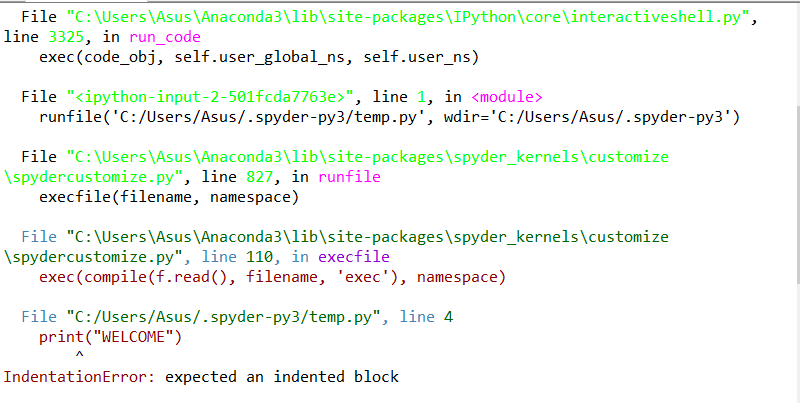
\includegraphics[scale=0.5]{Gambar/E2}
	\caption{Hasil Run}
\end{figure}
\\
\\
\\
\\
\\
\\
\\
\\
\\
\section{cara menangani errornya}
1. Lihat line berapa yang menandakan error , lalu tekan TAB atau spasi.
\begin{figure}[h]
	\centering
		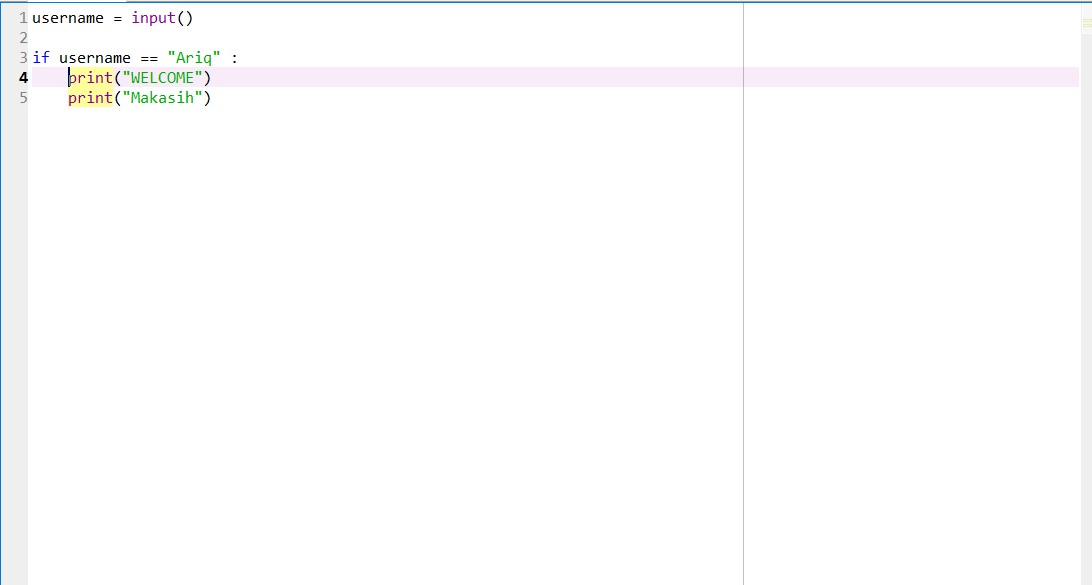
\includegraphics[scale=0.4]{Gambar/E3}
	\caption{Sudah Di Edit}
\end{figure}

\end{document}
